\documentclass[slidestop]{beamer}
\usepackage{beamerthemesplit}
\usepackage{graphics}
\usepackage{pstricks}

\graphicspath{{./}}

\title{The Libre-SOC Hybrid 3D CPU}
\author{Luke Kenneth Casson Leighton}


\begin{document}

\frame{
   \begin{center}
    \huge{The Libre-SOC Hybrid 3D CPU}\\
    \vspace{32pt}
    \Large{Augmenting the OpenPOWER ISA}\\
    \Large{to provide 3D and Video instructions}\\
    \Large{(properly and officially) and make a GPU}\\
    \vspace{24pt}
    \Large{FOSDEM2021}\\
    \vspace{16pt}
    \large{Sponsored by NLnet's PET Programme}\\
    \vspace{6pt}
    \large{\today}
  \end{center}
}


\frame{\frametitle{Why another SoC?}

 \begin{itemize}
   \item Intel Management Engine, Apple QA issues, Spectre\vspace{6pt}
   \item Endless proprietary drivers, "simplest" solution: \\
         License proprietary hard macros (with proprietary firmware)\\
   		 Adversely affects product development cost\\
   		due to opaque driver bugs (Samsung S3C6410 / S5P100)
   		 \vspace{6pt}
   \item Alternative: Intel and Valve-Steam collaboration\\
         "Most productive business meeting ever!"\\
         https://tinyurl.com/valve-steam-intel
		\vspace{6pt}
   \item Because for 30 years I Always Wanted To Design A CPU
		\vspace{6pt}
   \item Ultimately it is a strategic \textit{business} objective to
         develop entirely Libre hardware, firmware and drivers.
  \end{itemize}
}


\frame{\frametitle{Why OpenPOWER?}

\vspace{15pt}

 \begin{itemize}
   \item Good ecosystem essential\\
   		 linux kernel, u-boot, compilers, OSes,\\
   		 Reference Implementation(s)\vspace{10pt}
   \item Supportive Foundation and Members\\
   		 need to be able to submit ISA augmentations\\
   		 (for proper peer review)\vspace{10pt}
   \item No NDAs, full transparency must be acceptable\\
	     due to being funded under NLnet's PET Programme\vspace{10pt}
   \item OpenPOWER: established for decades, excellent Foundation,\\
   	     Microwatt as Reference, approachable and friendly.
  \end{itemize}
}

\frame{\frametitle{How can you help?}

\vspace{5pt}

 \begin{itemize}
   \item Start here! https://libre-soc.org \\
   	     Mailing lists https://lists.libre-soc.org \\
   	     IRC Freenode libre-soc \\
   	     etc. etc. (it's a Libre project, go figure) \\
		   \vspace{3pt}
   \item Can I get paid? Yes!  NLnet funded\\
   		 See https://libre-soc.org/nlnet/\#faq \\
   		 \vspace{3pt}
   \item Also profit-sharing in any commercial ventures \\
	     \vspace{3pt}
   \item How many opportunities to develop Libre SoCs exist,\\
   	     and actually get paid for it?
   	     	     \vspace{3pt}
   \item I'm not a developer, how can I help?\\
   		- Plenty of research needed, artwork, website \\
   		- Help find customers and OEMs willing to commit (LOI)
  \end{itemize}
}



\frame{\frametitle{What goes into a typical SoC?}
\vspace{9pt}
 \begin{itemize}
   \item 15 to 20mm BGA package: 2.5 to 5 watt power consumption\\
   		heat sink normally not required (simplifies overall design)
   		\vspace{3pt}
   \item Fully-integrated peripherals (not Northbridge/Southbridge)\\
         USB, HDMI, RGB/TTL, SD/MMC, I2C, UART, SPI, GPIO etc. etc. 
         \vspace{3pt}
   \item Built-in GPU (shared memory bus, 3rd party licensed) \vspace{3pt}
   \item Built-in VPU (likewise, proprietary)\vspace{3pt}
   \item Target price between \$2.50 and \$30 depending on market\\
         Radically different from IBM POWER9 Core (200 Watt)
         \vspace{3pt}
   \item We're doing the same, just with a hybrid architecture.\\
   		 CPU == GPU == VPU
  \end{itemize}
}



\frame{\frametitle{Simple SBC-style SoC}

\begin{center}
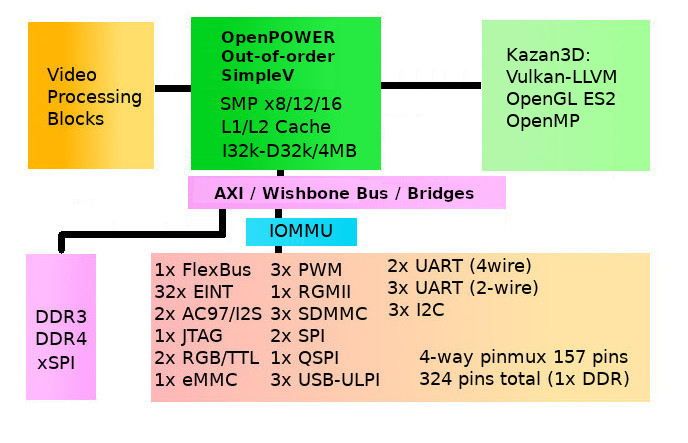
\includegraphics[width=0.9\textwidth]{shakti_libre_soc.jpg}
\end{center}

}

\frame{\frametitle{What's different about Libre-SOC?}

 \begin{itemize}
   \item Hybrid - integrated.  The CPU \textit{is} the GPU.\\
         The GPU \textit{is} the CPU.  The VPU \textit{is} the CPU.\\
         \textit{There is No Separate VPU/GPU Pipeline or Processor}\\
   		  \vspace{9pt}
   \item written in nmigen (a python-based HDL).  Not VHDL\\
   		  not Verilog (definitely not Chisel3/Scala)\\
   		  This is an extremely important strategic decision.\\
   		  \vspace{9pt}
   \item Simple-V Vector Extension.  See `SIMD Considered harmful'.\\
   		  https://tinyurl.com/simd-considered-harmful\\   
   		SV effectively a "hardware for-loop" on standard scalar ISA\\
   		(conceptually similar to Zero-Overhead Loops in DSPs)
   		  \vspace{6pt}
   \item Yes great, but what's different compared to Intel, AMD, NVIDIA,
         ARM and IBM?
  \end{itemize}
}

\frame{\frametitle{OpenPOWER Cell Processor and upwards}

 \begin{itemize}
   \item OpenPOWER ISA developed from PowerPC, with the RS6000 in the 90s.
   		  \vspace{6pt}
   \item Sony, IBM and Toshiba began the Cell Processor in 2001 \\
   		  (Sony Playstation 3) - NUMA approach
   		  \vspace{6pt}
   \item Raw brute-force performance pissed all over the competition
         at the time
   		  \vspace{6pt}
   \item VSX later evolved out of this initiative.
   		  \vspace{6pt}
   \item VSX, a SIMD extension, now showing its age.  \\
         Fixed-width, no predication, limited pixel formats (15 bit)
   		  \vspace{6pt}
   \item (Vulkan requires dozens of pixel formats)
  \end{itemize}
}

\frame{\frametitle{Apple M1 (ARM) vs Intel / AMD (x86)}

 \begin{itemize}
   \item Very interesting article: tinyurl.com/apple-m1-review
   \item Apple M1: uses ARM.  Intel: implements x86
   \item Apple M1: RISC multi-issue.  Intel: CISC multi-issue.
   \item Apple M1: uniform (easy) instruction decode \\
         Intel: \textit{Cannot easily identify start of instruction}
   \item Result: multi-issue x86 decoder is so complex, it misses
         opportunities to keep back-end execution engines 100 percent
         occupied
   \item OpenPOWER happens to be RISC (easy decode), which is why POWER10
         has 8-way multi-issue.
   \item Libre-SOC can do the same tricks that IBM POWER10 and Apple M1
         can.  Intel (x86) literally cannot keep up.
  \end{itemize}
}


\frame{\frametitle{Hybrid Architecture: Augmented 6600}

 \begin{itemize}
   \item CDC 6600 is a design from 1965.  The \textit{augmentations} are not.\\
   		 Help from Mitch Alsup includes \textit{precise exceptions}, \\
   		 multi-issue and more. Academic literature on 6600 utterly misleading.
   		6600 Scoreboards completely underestimated (Seymour Cray and
   		James Thornton
   		solved problems they didn't realise existed elsewhere!)
   \item Front-end Vector ISA, back-end "Predicated (masked) SIMD"\\
         nmigen (python OO) strategically critical to achieving this.
   \item Out-of-order combined with Simple-V allows scalar operations\\
         at the developer end to be turned into SIMD at the back-end\\
         \textit{without the developer needing to do SIMD}
   \item IEEE754 sin / cos / atan2, Texturisation opcodes, YUV2RGB\\
   		 all automatically vectorised.
  \end{itemize}
}

\frame{\frametitle{Learning from these and putting it together}

 \begin{itemize}
   \item Apple M1 and IBM POWER10 show that RISC plus superscalar
         multi-issue produces insane performance
   \item Intel AVX 512 and CISC in general is getting out of hand (what's
         next: 256-bit length instructions, AVX 1024?)
   \item RISC-V RVV shows Cray-style Vectors can save power.  Simple-V
         has the same benefits with far less instructions (188 for RVV,
         3 to 5 new instructions for Simple-V).
   \item CDC 6600 shows that intelligently-implemented designs can do the
         job, with far less resources.
   \item Libre-SOC combines the best of historical processor designs,
         co-opting and innovating on them (pissing in the back yard of
         every incumbent CPU and GPU company in the process).
   \item It's a Libre project: you get to help
  \end{itemize}
}


\frame{\frametitle{Why nmigen?}

 \begin{itemize}
   \item Uses python to build an AST (Abstract Syntax Tree).
         Actually hands that over to yosys (to create ILANG file)
         after which verilog can (if necessary) be created
   \item Deterministic synthesiseable behaviour (Signals are declared
         with their reset pattern: no more forgetting "if rst" block).
   \item python OO programming techniques can be deployed.  classes
         and functions created which pass in parameters which change
         what HDL is created (IEEE754 FP16 / 32 / 64 for example)
   \item python-based for-loops can e.g. read CSV files then generate
         a hierarchical nested suite of HDL Switch / Case statements
         (this is how the Libre-soc PowerISA decoder is implemented)
   \item extreme OO abstraction can even be used to create "dynamic
         partitioned Signals" that have the same operator-overloaded
         "add", "subtract", "greater-than" operators
   
  \end{itemize}
}

\frame{\frametitle{Why another Vector ISA? (or: not-exactly another)}

 \begin{itemize}
   \item Simple-V is a 'register tag' system.  \textit{There are no opcodes}\\
   		 SV 'tags' scalar operations (scalar regfiles) as 'vectorised'
   \item (PowerISA SIMD is around 700 opcodes, making it unlikely to be
    	 able to fit a PowerISA decoder in only one clock cycle)
   \item Effectively a 'hardware sub-counter for-loop': pauses the PC\\
         then rolls incrementally through the operand register numbers\\
         issuing \textit{multiple} scalar instructions into the pipelines\\
         (hence the reason for a multi-issue OoO microarchitecture)
   \item Current \textit{and future} PowerISA scalar opcodes inherently
   	 	 \textit{and automatically} become 'vectorised' by SV without
   	 	 needing an explicit new Vector opcode.
   \item Predication and element width polymorphism are also 'tags'.
         elwidth polymorphism allows for BF16 / FP16 / 80 / 128 to be added to
         the ISA \textit{without modifying the ISA}
   
  \end{itemize}
}

\frame{\frametitle{Quick refresher on SIMD}

 \begin{itemize}
   \item SIMD very easy to implement (and very seductive)
   \item Parallelism is in the ALU
   \item Zero-to-Negligeable impact for rest of core
  \end{itemize}
  Where SIMD Goes Wrong:\vspace{6pt}
   \begin{itemize}
   \item See "SIMD instructions considered harmful"
   https://sigarch.org/simd-instructions-considered-harmful
   \item Setup and corner-cases alone are extremely complex.\\
         Hardware is easy, but software is hell.\\
         strncpy VSX patch for POWER9: 250 hand-written asm lines!\\
         (RVV / SimpleV strncpy is 14 instructions)
   \item O($N^{6}$) ISA opcode proliferation (1000s of instructions)\\
         opcode, elwidth, veclen, src1-src2-dest hi/lo
  \end{itemize}
}

\begin{frame}[fragile]
\frametitle{Simple-V ADD in a nutshell}

\begin{semiverbatim}
function op\_add(rd, rs1, rs2, predr) # add not VADD!
  int i, id=0, irs1=0, irs2=0;
  for (i = 0; i < VL; i++)
    if (ireg[predr] & 1<<i) # predication uses intregs
       ireg[rd+id] <= ireg[rs1+irs1] + ireg[rs2+irs2];
    if (reg\_is\_vectorised[rd] )  \{ id += 1; \}
    if (reg\_is\_vectorised[rs1])  \{ irs1 += 1; \}
    if (reg\_is\_vectorised[rs2])  \{ irs2 += 1; \}
\end{semiverbatim}

  \begin{itemize}
   \item Above is oversimplified: Reg. indirection left out (for clarity).
   \item SIMD slightly more complex (case above is elwidth = default)
   \item Scalar-scalar and scalar-vector and vector-vector now all in one
   \item OoO may choose to push ADDs into instr. queue (v. busy!)
  \end{itemize}
\end{frame}

\frame{\frametitle{Additional Simple-V features}

 \begin{itemize}
   \item "fail-on-first" (POWER9 VSX strncpy segfaults on boundary!)
   \item "Twin Predication" (covers VSPLAT, VGATHER, VSCATTER, VINDEX etc.)
   \item SVP64: extensive "tag" (Vector context) augmentation
   \item "Context propagation": a VLIW-like context.  Allows contexts
         to be repeatedly applied.
          Effectively a "hardware compression algorithm" for ISAs.
   \item Ultimate goal: cut down I-Cache usage, cuts down on power
   \item Typical GPU has its own I-Cache and small shaders.\\
        \textit{We are a Hybrid CPU/GPU: I-Cache is not separate!}
   \item Needs to go through OpenPOWER Foundation `approval'         
  \end{itemize}
}


\frame{\frametitle{Summary}

 \begin{itemize}
   \item Goal is to create a mass-volume low-power embedded SoC suitable
         for use in netbooks, chromebooks, tablets, smartphones, IoT SBCs.
   \item No way we could implement a project of this magnitude without
         nmigen (being able to use python OO to  HDL)
   \item Collaboration with OpenPOWER Foundation and Members absolutely
         essential. No short-cuts.  Standards to be developed and ratified
         so that everyone benefits.
   \item Riding the wave of huge stability of OpenPOWER ecosystem
   \item Greatly simplified open 3D and Video drivers reduces product
         development costs for customers
   \item It also happens to be fascinating, deeply rewarding technically
         challenging, and funded by NLnet
         
  \end{itemize}
}


\frame{
  \begin{center}
    {\Huge The end\vspace{12pt}\\
		   Thank you\vspace{12pt}\\
		   Questions?\vspace{12pt}
	}
  \end{center}
  
  \begin{itemize}
	\item Discussion: http://lists.libre-soc.org
	\item Freenode IRC \#libre-soc
	\item http://libre-soc.org/
	\item http://nlnet.nl/PET
	\item https://libre-soc.org/nlnet/\#faq
  \end{itemize}
}


\end{document}
